\documentclass{article}
\usepackage[a4paper, total={6in, 8in}]{geometry}
\usepackage{graphicx} % Required for inserting images
\usepackage{amssymb}
\usepackage{amsmath}
\usepackage{amsfonts}
\usepackage{extarrows}
\usepackage{soul}
\usepackage{enumitem}
\usepackage{varwidth}
\usepackage[T1]{fontenc}
\tolerance=1
\emergencystretch=\maxdimen
\hyphenpenalty=10000
\hbadness=10000

\author{}
\date{}
\title{Quantique TD3 : Fonction d'onde - Équation de Schr$\ddot{o}$dinguer}

\begin{document}
\maketitle

\noindent\textbf{Ex1: Fonction d'onde - Probabilité de présence}\newline
On étudie une particule dont la fonction d'onde, définie $\forall x \in [0;+\infty[$, vaut:
\[ \psi(x) = \psi_{0}e^{-\frac{x}{x_{0}}}\] où $x_{0}$ est une constante fixée et $\psi_{0}$ est une constante à déterminer.
\begin{enumerate}
    \item Donner la fonction de répartition de probabilité de présence de la particule pour x$\in [0;+\infty[$ en fonction de $\psi_{0}$, $x_{0}$ et x.\newline
    La fonction de répartiton de probabilité de présence de la particule pour x$\in$[0;$+\infty$[ est: P = $\int_{0}^{\infty} |\psi(x)|^{2}dx$ avec $|\psi(x)|^{2}$ la densité de probabilité de présence.
    \begin{flalign*}
        P & = \int_{0}^{\infty} \psi_{0}^{2} e^{-\frac{2x}{x_{0}}} dx&\\
          & = \psi_{0}^{2} \left[-\frac{x_{0}}{2} e^{-\frac{2x}{x_{0}}}\right]_{0}^{+\infty}&\\
          & = \psi_{0}^{2} \left(\frac{-x_{0}}{2}\right) \left(\lim_{x\to\infty} e^{-\frac{2x}{x_{0}}} - e^{0}\right)&\\
          & = \psi_{0}^{2} \left(-\frac{x_{0}}{2}\right)(0-1)&\\
        P & = \psi_{0}^{2} \frac{x_{0}}{2} 
    \end{flalign*}
    \item En utilisant la condition de normalisation de la fonction d'onde, déterminer la valeur de la constante $\psi_{0}$.\newline
    Condition de normalisation : P = 1 (dans l'espace [0;+$\infty$[) donc :
    \[ \psi_{0}^{2} \frac{x_{0}}{2} = 1 \Longleftrightarrow \psi_{0}^{2} = \frac{2}{x_{0}}  \Longleftrightarrow \psi_{0} = \sqrt{\frac{2}{x_{0}}}; x_{0}>0 \]
    \item Quelle est la probabilité de trouver la particule dans l'intervalle [0;A]?
    \begin{flalign*}
        P_{[0;A]} & = \int_{0}^{A} |\psi(x)|^{2}dx&\\
                  & = \int_{0}^{A} \psi_{0}^{2} e^{-\frac{2x}{x_{0}}}dx&\\
                  & = \int_{0}^{A} \frac{2}{x_{0}} \times e^{-\frac{2x}{x_{0}}}dx&\\
                  & = \frac{2}{x_{0}} \left[-\frac{x_{0}}{2} (e^{-\frac{2x}{x_{0}}})\right]_{0}^{A}&\\
                  & = -1 \left[e^{-\frac{2A}{x_{0}}}-1\right]&\\
                  & = 1 - e^{-\frac{2A}{x_{0}}}
    \end{flalign*}
    \item Que doit valoir A pour que cette probabilité soit au minimum de 95 $\%$ ? On donnera en fonction de $x_{0}$ un résultat approché en prenant \ln(0,05) $\approx$ -3.
    \begin{flalign*}
        P \geqslant 95\% & \Longleftrightarrow 1 - e^{-\frac{2A}{x_{0}}} \geqslant 0,95 &\\
                         & \Longleftrightarrow  e^{-\frac{2A}{x_{0}}}-1 \leqslant -0,95 &\\
                         & \Longleftrightarrow e^{-\frac{2A}{x_{0}}} \leqslant 0,05 &\\
                         & \Longleftrightarrow \ln\left(e^{-\frac{2A}{x_{0}}}\right) \leqslant \ln(0,05) &\\
                         & \Longleftrightarrow -\frac{2A}{x_{0}} \leqslant -3 &\\
                         & \Longleftrightarrow A \approx \frac{3x_{0}}{2}
    \end{flalign*}
\end{enumerate}

\noindent\textbf{Ex2: Particule dans un puits de potentiel infini}\newline
On étudie une particule de masse m dans le puits de potentiel infini suivant:
\[V(x) = \left\{
    \begin{array}{c}
        \text{0 si x } \in [0;L] \\
        +\infty \text{ sinon}
    \end{array}
\]

On veut connaitre les états d'énergie accessibles à la particule, ainsi que l'allure des fonctions d'onde associées à chaque niveau d'énergie.
\begin{figure}[h]
    \centering
    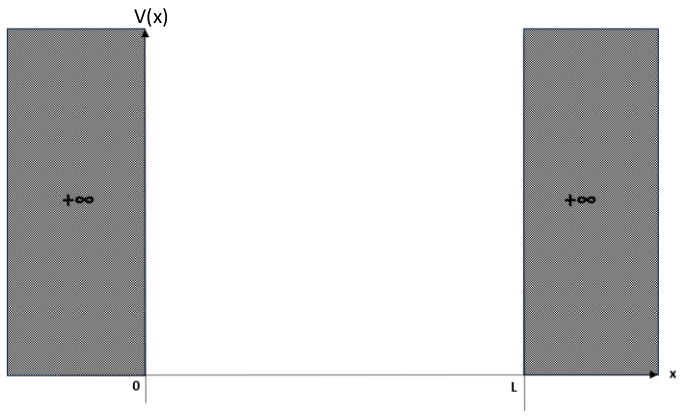
\includegraphics[scale=0.3]{figure1.png}
    \caption{Puits de potentiel infini de largeur L}
\end{figure}

\begin{enumerate}
    \item Pour x $\in$ [0;L], donner l'équation de Schr$\ddot{o}$dinguer vérifiée par la fonction d'onde $\psi$ de la particule dans le puits de potentiel infini, en fonction de la constante de Planck réduite à $\hbar$ ($\hbar = \frac{h}{2\pi}$), de m et de l'énergie E de la particule.
    \item Donner la forme générale des solutions $\psi$(x) de l'équation de Schr$\ddot{o}$dinger sur ce domaine.
    \item Quelles sont les conditions aux limites $\psi$(0) et $\psi$(L)? Utiliser ces conditions pour déterminer certaines des constantes de la solution générale $\psi$(x).
    \item Quel vaut $\int_{0}^{L} |\psi(x)|^{2}dx$ ? Utiliser ce résultat pour déterminer complètement l'expression de $\psi$(x).
    \item Reporter ce résultat dans l’équation de Schr$\ddot{o}$dinger pour déterminer les valeurs d’énergie accessibles à la particule. Comment interprétez-vous ce résultat ? Quel facteur de l’expression peut être qualifié de "nombre quantique" associé au niveau d’énergie ?
    \item Schématiser le diagramme d’énergie en traçant sur chaque niveau l’allure de la fonction de probabilité de présence $|\psi(x)|^{2}$ pour x $\in$ [0;L].
\end{enumerate}

\noindent\textbf{Ex3: Boîte quantique}\newline
On s’intéresse maintenant au puits quantique 3D : la boîte quantique. La fonction d’onde $\psi$(x, y, z) associée à une particule de masse m présente dans la boîte est alors fonction des trois variables de l’espace. Le potentiel V(x, y, z) est nul dans la boîte, infini en-dehors :
\[ V(x,y,z)= \left\{
    \begin{array}{c}
        0 \text{ si } (x,y,z) \in [0;a] \times [0;b] \times [0;c] \\
        +\infty \text{ sinon}
    \end{array}
\]

\begin{figure}[h]
    \centering
    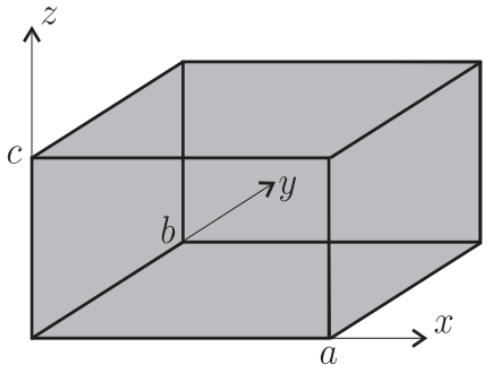
\includegraphics[scale=0.3]{figure2.png}
    \caption{Boîte quantique de dimensions a$\times$b$\times$c}
\end{figure}

\begin{enumerate}
    \item Rappeler l’équation de Schr$\ddot{o}$dinger appliquée à $\psi$ en fonction de $\hbar$, m, de l’énergie E de la particule et des dérivées partielles secondes spatiales de $\psi$.

    \newline\newline De manière analogue au cas 1D, on montre que:
    \[ \psi(x,y,z) = \sqrt{\frac{8}{abc}}\sin\left(\frac{n\pi}{a}x\right) \sin\left(\frac{p\pi}{b}y\right) \sin\left(\frac{q\pi}{c}z\right) \]

    \item Identifier les facteurs pouvant être qualifiés de nombres quantiques associés à chaque niveau d’énergie.
    \item Utiliser l’équation de Schr$\ddot{o}$dinger pour déterminer les niveaux d’énergie accessibles en fonction notamment des nombres quantiques.
    \item Pour le cas particulier a = b = c, donner l’expression du plus petit niveau d’énergie $E_{f}$ en fonction de $\hbar$, m et a. Pour quelles valeurs des nombres quantiques ce niveau est-il atteint ?
    \item Lorsque N jeux de nombres quantiques permettent d’atteindre un même niveau d’énergie, l’on dit ce niveau d’énergie est de degré de dégénérescence N. Compléter le tableau suivant pour les trois premiers niveaux d’énergie. Donner leur énergie en fonction de $E_{f}$.\newline\newline
    \begin{centering}
        \begin{tabular}{|c|c|c|c|}
            \hline
            Niveau & Nombres quantiques & Énergie & Degré de dégénérescence N \\
            \hline
            1 & & & \\
            \hline
            2 & & & \\
            \hline
            3 & & & \\
            \hline
        \end{tabular}
    \end{centering}\newline\newline
    \textit{Rappel : opérateur laplacien scalaire en coordonnées cartésiennes :}
    \[ 1D : \Delta = \frac{d^{2}}{dx^{2}}; 3D : \Delta = \frac{\delta^{2}}{\delta x^{2}} + \frac{\delta^{2}}{\delta y^{2}} + \frac{\delta^{2}}{\delta z^{2}} \]
\end{enumerate}

\newpage
\noindent\textbf{Notes de cours}\newline
L'équation de Schrodinguer est équivalente au PFD.
\[
    H\psi = E\psi
    \quad
    \begin{varwidth}{\displaywidth}
        \begin{itemize}[nosep]
            \item H = $-\frac{\hbar^{2}}{2m}\Delta + V$: opérateur Hamiltonien
            \item E: opérateur 
        \end{itemize}
    \end{varwidth}
\]

Pour rappel : $\Delta$ est l'opérateur Laplacien qui correspond à la somme des dérivés secondes partielles de chaque variables.\newline

$-\frac{\hbar^{2}}{2m}\Delta\psi + V\psi = E\psi$ qui donne $\psi$(x,y,z,t) = fonction d'onde qui caractérise l'état de la particule donc donne:\newline
$\left\{
    \begin{array}{l}
        \text{la probabilité de présence} \\
        \text{l'énergie de la particule}
    \end{array}    
$\newline\newline
$\left\{
    \begin{array}{l}
        \text{état stationnaire} \Longrightarrow \psi(x,y,z) \\
        \text{système à une dimension} \Longrightarrow \psi(x)
    \end{array}    
$
\newline
On en conclut donc que l'équation de Schrodinguer à l'état stationnaire et à une dimension :
\[
    -\frac{\hbar^{2}}{2m}\frac{d^{2}}{dx^{2}}\psi(x) + V\psi(x) = E\psi(x)    
\]
On note que c'est une dérivé totale car dérivé partielle mais il n'y a qu'une variable.\newline

La densité de probabilité de présence dP se calcule ainsi : dP = $|\psi (x)|^{2}$dx qui correspond au carré du module de la fonction d'onde $\psi(x)$.\newline

La répartition de la probabilité de présence dans une intervalle donné P se calcule ainsi : $\int_{a}^{b}|\psi(x)|^{2}dx$.\newline

La condition de la normalisation (probabilité de trouver la particule dans l'espace (]-$\infty$;+$\infty$[):\newline P = 1 = $\int_{-\infty}^{+\infty}|\psi(x)|^{2}dx$
\end{document}
